\chapter{Overview}

T2SP generates accelerators for dense tensor computes, and a general workflow is shown in Fig.~\ref{fig:overall-flow}. Usually, such a compute is described as one or a few math equations.  We can rewrite these equations to be recursive, the so-called Uniform Recursive Equations or UREs. With UREs, we can accurately control input and output data to flow in a pipeline fashion during the compute.

We can write basic UREs without tiling the compute domain. Then we tile the compute domain for data locality and reuse. Correspondingly, we need translate the basic UREs into final UREs after tiling, which is straightforward.

UREs can be expressed in C/C++. After adding some helper code necessary for testing,  we can compile them in a standard C/C++ compiler, and check if the UREs are correct vs. the original math equations.

The compute domain is iterated with a loop nest. If the compute is to run on a GPU, we need decide which loops are block loops, and inside a block, which loops are thread loops: An iteration of the thread loops will be turned into a thread. If the compute is to run on an FPGA, however, we always use a single thread for the entire compute, and thus there is no block or thread loop. 

Inside a thread, we will build a systolic array in a space-time transform. So we need decide which loops are space loops.  

Finally, we add an I/O network for the systolic array.  The I/O network is composed of multiple memory levels. The input/output data are loaded/unloaded through the I/O network into/out of the systolic array. Once in the systolic array, the data flow through the array according to the UREs.  

Now for the original compute, we have a complete T2SP program, or more accurately, a specification, since such a program only specifies what to implement (e.g. space-time transform and I/O network), but leave the actual implementation to the T2SP compiler. In other words, the program controls the compiler to generate the expected accelerator. 

For an FPGA, the T2SP compiler generates OpenCL device code and a C interface, compile and run these generated code by invoking the downstream FPGA tools. The programmer can use the emulator tool to verify correctness of the generated code, and use the synthesis tool to produce a bit-stream.  The programmer can write CPU host code and call the device code through the C interface, just like calling any normal C function on a CPU. That call would offload the compute to the emulator or an actual FPGA to run.

For a GPU, the T2SP compiler generates CM device code, and invoke the CM compiler to build a binary. The programmer need write CPU host code that offloads the device code to a GPU. 

A beginner might encounter several hurdles in using T2SP: (1) how to write UREs? (2) how to tile loops? (3) how to decide block, thread, and space loops? and (4) how to design I/O? There are numerous valid answers for each of these questions. Fortunately, we do not have to be mathematicians, algorithm experts, or computer architects in order to effectively address the questions. Based on intuitive rules, any programmer may master some simple programming skills quickly, and  use the skills to accelerate real-world workloads.

We will describe the steps in more details below. 

\begin{figure}[!ht]
    \centering
    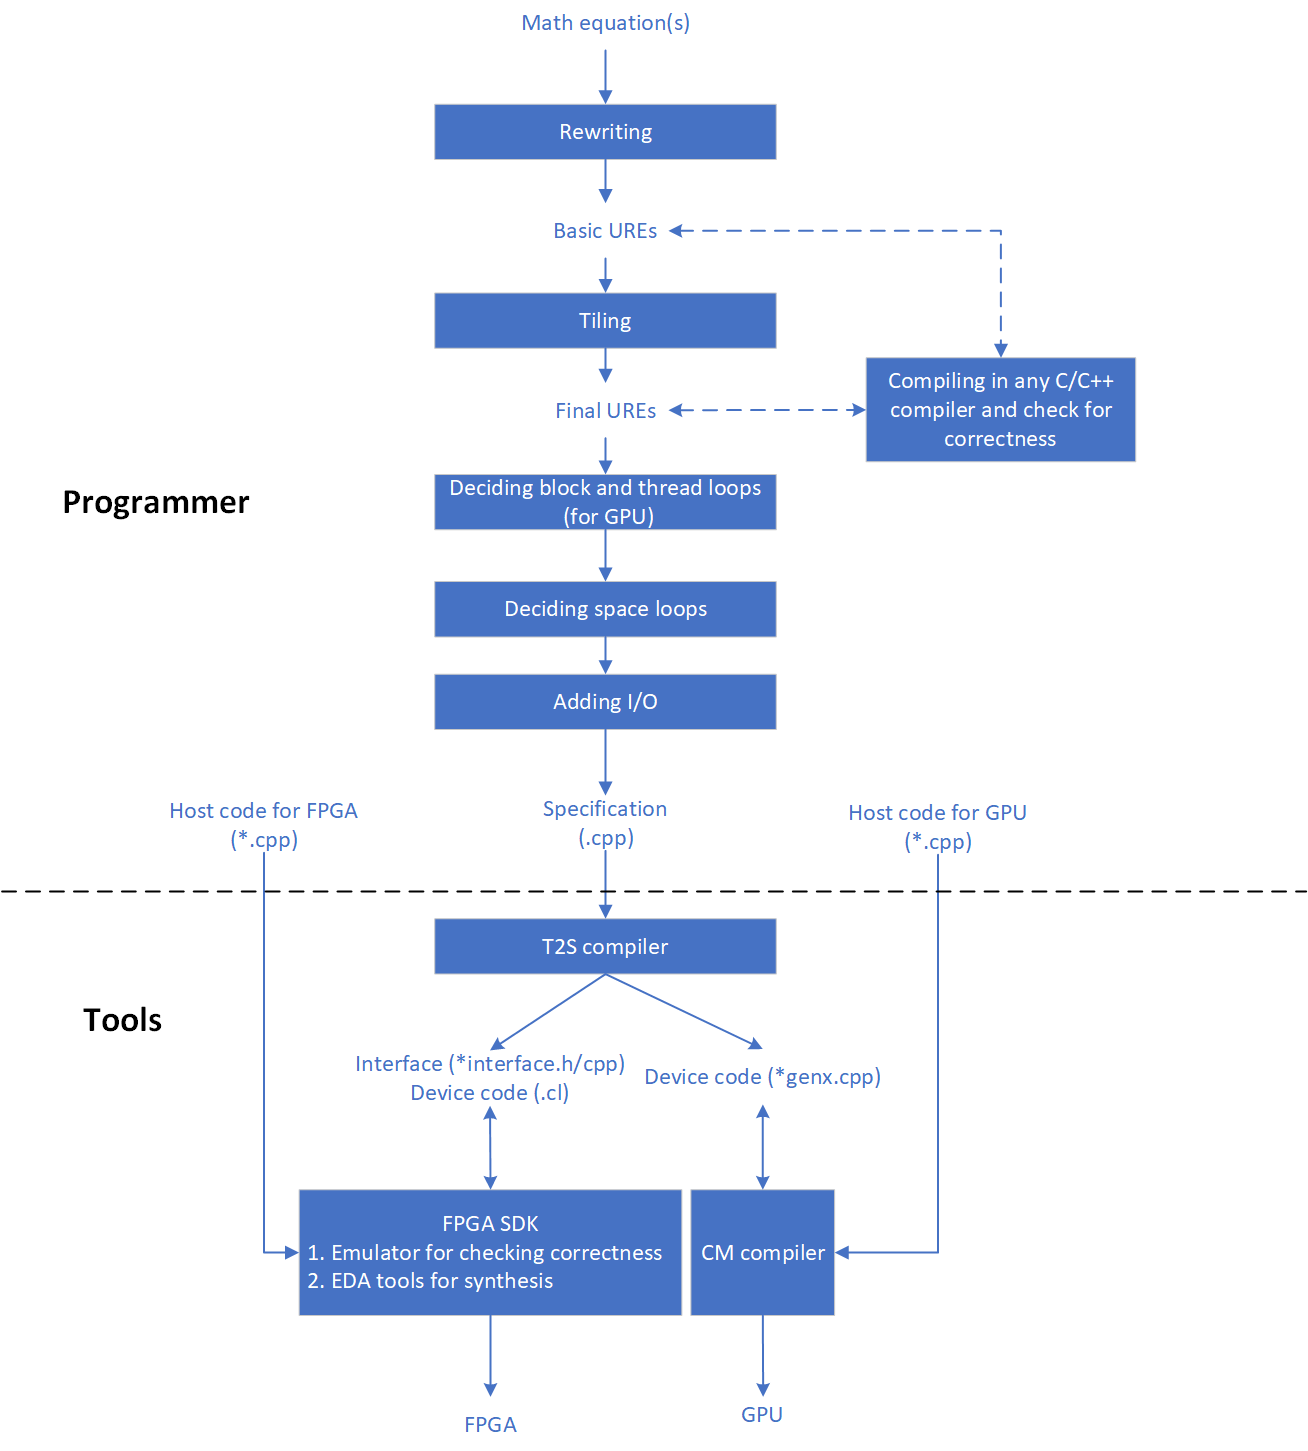
\includegraphics[width=\textwidth]{img/overall-flow.png}
    \caption{Overall flow}
    \label{fig:overall-flow}
\end{figure}
